\documentclass[12pt,a4paper]{article}
\usepackage[utf8]{inputenc}
\usepackage[T1]{fontenc}
\usepackage{lmodern}
\usepackage{microtype}
\usepackage[margin=2.2cm]{geometry}
\usepackage{amsmath,amssymb}
\usepackage{icomma}
\usepackage{xcolor}
\usepackage{booktabs,array}
\usepackage{enumitem}
\usepackage{fancyhdr}
\usepackage[most]{tcolorbox}
\usepackage{tikz}
\usetikzlibrary{arrows.meta,positioning,shapes.geometric}
\usepackage{pgfplots}
\pgfplotsset{compat=1.18}
\usepackage[hidelinks]{hyperref}

\setlength{\parindent}{0pt}
\setlength{\parskip}{6pt}
\renewcommand{\contentsname}{Sumário}

% ---------- cores ----------
\definecolor{azul}{HTML}{1F4E79}
\definecolor{verde}{HTML}{2E7D32}
\definecolor{laranja}{HTML}{E65100}
\definecolor{vermelho}{HTML}{C62828}
\definecolor{cinza}{HTML}{F3F4F6}

\pagestyle{fancy}
\fancyhf{}
\lhead{\small Revisão Prova 3 -- Sistemas de Informação}
\rhead{\small Resolução passo a passo}
\cfoot{\thepage}

% ---------- caixas ----------
\newtcolorbox{enunciado}{colback=cinza,colframe=azul,fonttitle=\bfseries,title=Enunciado,breakable}
\newtcolorbox{dados}{colback=azul!5,colframe=azul,fonttitle=\bfseries,title=Passo 1 -- Separe os dados (o que o problema me deu?)}
\newtcolorbox{passo}[1]{colback=white,colframe=azul!70,fonttitle=\bfseries,title={#1},breakable}
\newtcolorbox{resultado}{colback=verde!8,colframe=verde,fonttitle=\bfseries,title=Resposta final}
\newtcolorbox{interpreta}{colback=laranja!6,colframe=laranja,fonttitle=\bfseries,title=Interpretação em linguagem simples}
\newtcolorbox{cuidado}{colback=vermelho!5,colframe=vermelho,fonttitle=\bfseries,title=Cuidado! Erro comum}
\newtcolorbox{traducao}{colback=white,colframe=laranja!80,fonttitle=\bfseries,title=Traduzindo o problema para o português do dia a dia}

\pgfmathdeclarefunction{gauss}{1}{\pgfmathparse{exp(-(#1)^2/2)/sqrt(2*pi)}}

% ---------- desenho: reta do intervalo ----------
% #1 = limite inferior, #2 = centro, #3 = limite superior, #4 = margem, #5 = nome do centro
\newcommand{\ICline}[5]{%
\begin{center}
\begin{tikzpicture}[font=\small]
  \draw[-{Latex},thick] (-0.8,0) -- (8.8,0);
  \fill[verde!20] (1,-0.22) rectangle (7,0.22);
  \draw[very thick,verde] (1,-0.4) -- (1,0.4);
  \draw[very thick,verde] (7,-0.4) -- (7,0.4);
  \fill[azul] (4,0) circle (3.5pt);
  \draw[{Latex}-{Latex}] (1,0.75) -- (4,0.75) node[midway,above] {$-\,E = -\,#4$};
  \draw[{Latex}-{Latex}] (4,0.75) -- (7,0.75) node[midway,above] {$+\,E = +\,#4$};
  \node[below=7pt] at (1,0) {$\mathbf{#1}$};
  \node[below=7pt] at (4,0) {$\mathbf{#2}$};
  \node[below=7pt] at (7,0) {$\mathbf{#3}$};
  \node[below=24pt,align=center] at (1,0) {limite\\inferior};
  \node[below=24pt,align=center] at (4,0) {#5\\(centro)};
  \node[below=24pt,align=center] at (7,0) {limite\\superior};
\end{tikzpicture}
\end{center}}

% ---------- desenho: curva com regiões de rejeição ----------
% #1 = valor crítico, #2 = estatística calculada, #3 = rótulo da estatística, #4 = rótulo do crítico
\newcommand{\RejCurve}[4]{%
\begin{center}
\begin{tikzpicture}
\begin{axis}[width=13cm,height=6cm,axis lines=middle,ymin=0,ymax=0.48,xmin=-4,xmax=4,
  ytick=\empty,xtick={-#1,0,#1},
  xticklabels={{$-#4$},{$0$},{$+#4$}},
  every axis x label/.style={at={(current axis.right of origin)},anchor=west},
  clip=false]
  \addplot[fill=vermelho!35,draw=none,domain=-4:-#1,samples=50] {gauss(x)} \closedcycle;
  \addplot[fill=vermelho!35,draw=none,domain=#1:4,samples=50] {gauss(x)} \closedcycle;
  \addplot[fill=verde!20,draw=none,domain=-#1:#1,samples=80] {gauss(x)} \closedcycle;
  \addplot[thick,azul,domain=-4:4,samples=120] {gauss(x)};
  \node[align=center,font=\small] at (axis cs:0,0.17) {NÃO rejeito $H_0$\\(região do\\``normal'')};
  \node[align=center,font=\small,vermelho] at (axis cs:-3.2,0.17) {Rejeito\\$H_0$\\(2,5\%)};
  \node[align=center,font=\small,vermelho] at (axis cs:3.45,0.17) {Rejeito\\$H_0$\\(2,5\%)};
  \draw[very thick,laranja,-{Latex}] (axis cs:#2,0.36) -- (axis cs:#2,0.005);
  \node[laranja,font=\bfseries\small,above] at (axis cs:#2,0.36) {#3};
\end{axis}
\end{tikzpicture}
\end{center}}

\begin{document}

% ================= CAPA =================
\begin{center}
{\Huge\bfseries\color{azul} Revisão da Prova 3}\\[6pt]
{\Large Intervalos de confiança e testes de hipóteses}\\[4pt]
{\large Resolução passo a passo, para quem nunca viu o conteúdo}\\[4pt]
{\normalsize Usando o mesmo método da professora (Sistemas de Informação -- 2026)}
\end{center}

\begin{tcolorbox}[colback=azul!5,colframe=azul,title=Como usar este material]
\begin{enumerate}[leftmargin=*,itemsep=2pt]
  \item Leia a \textbf{Parte 0} (3 páginas). Ela explica cada símbolo, em português simples.
  \item Use o \textbf{mapa de decisão} (página \pageref{mapa}) para saber qual fórmula usar.
  \item Faça os exercícios na ordem. Todos seguem a mesma receita:\\
  \textbf{separar os dados} $\rightarrow$ \textbf{escolher a fórmula} $\rightarrow$ \textbf{fazer uma conta por vez} $\rightarrow$ \textbf{escrever a conclusão}.
  \item Na véspera da prova, refaça cada exercício \textbf{sem olhar} e confira com a resposta final.
\end{enumerate}
\textbf{Dica de calculadora:} use pelo menos \textbf{4 casas decimais} nas contas do meio e arredonde \textbf{só no final}.
\end{tcolorbox}

\tableofcontents

\newpage
% ================= PARTE 0 =================
\section*{Parte 0 -- O mínimo que você precisa saber}
\addcontentsline{toc}{section}{Parte 0 -- O mínimo que você precisa saber}

\subsection*{A ideia em uma frase}
Não dá para medir \textbf{todo mundo} (a \textbf{população}). Então medimos \textbf{alguns} (a \textbf{amostra}) e usamos esse resultado para dizer algo sobre todo mundo, \textbf{com uma margem de erro}.

\begin{tcolorbox}[colback=laranja!6,colframe=laranja,title=Analogia da sopa]
Para saber se uma panela de sopa está salgada, você não bebe a panela inteira: prova \textbf{uma colher} (amostra). Se a sopa foi bem mexida (amostra \textbf{aleatória}), a colher representa a panela (população).
\end{tcolorbox}

\subsection*{Dicionário dos símbolos (como se lê e o que significa)}
\renewcommand{\arraystretch}{1.35}
\begin{center}
\begin{tabular}{>{\centering\arraybackslash}m{1.6cm} m{3.2cm} m{10cm}}
\toprule
\textbf{Símbolo} & \textbf{Como se lê} & \textbf{O que significa} \\
\midrule
$n$ & ``ene'' & Tamanho da amostra: quantas pessoas ou coisas foram medidas. \\
$\bar{x}$ & ``xis barra'' & Média da \textbf{amostra} (o que calculamos com os dados). \\
$\mu$ & ``mi'' & Média da \textbf{população} (o valor verdadeiro, que queremos descobrir). \\
$\sigma$ & ``sigma'' & Desvio-padrão da \textbf{população}. Só usamos quando o enunciado diz que é \textbf{conhecido}. \\
$s$ & ``esse'' & Desvio-padrão da \textbf{amostra}. Mede o quanto os dados variam. \\
$\sqrt{\ }$ & ``raiz quadrada'' & Tecla $\sqrt{\ }$ da calculadora. Ex.: $\sqrt{64}=8$, porque $8\times 8=64$. \\
$\hat{p}$ & ``p chapéu'' & Proporção na amostra: $\hat{p}=\dfrac{x}{n}$ (quantos têm a característica, dividido pelo total). \\
$\alpha$ & ``alfa'' & Nível de significância. Na prova: $\alpha = 0,05 = 5\%$. \\
$E$ & ``margem de erro'' & Quanto somamos e subtraímos da média para montar o intervalo. \\
$gl$ & ``graus de liberdade'' & Um número que diz em qual \textbf{linha} da tabela $t$ olhar. \\
$H_0$ & ``agá zero'' & Hipótese nula: ``\textbf{não há diferença}'' (as médias são iguais). \\
$H_1$ & ``agá um'' & Hipótese alternativa: ``\textbf{há diferença}'' (as médias são diferentes). \\
\bottomrule
\end{tabular}
\end{center}

\subsection*{Os 3 nomes que sempre aparecem}
\begin{enumerate}[leftmargin=*]
  \item \textbf{Erro-padrão (EP):} quanto a média da amostra costuma ``oscilar''. É sempre
  \[ EP = \frac{\text{desvio-padrão}}{\sqrt{n}} \qquad(\text{o desvio dividido pela raiz de } n). \]
  \item \textbf{Valor crítico:} um número tirado da tabela. Para 95\%: \textbf{1,96} (tabela Z) ou o valor da tabela $t$.
  \item \textbf{Margem de erro:} $E = \text{valor crítico} \times EP$.
\end{enumerate}

\begin{tcolorbox}[colback=verde!8,colframe=verde,title=A receita de TODO intervalo de confiança]
\[
\boxed{\ \text{IC} = \text{estimativa} \pm E \qquad\text{onde}\qquad E = \text{valor crítico}\times EP\ }
\]
\textbf{Limite inferior} = estimativa $-\,E$ \qquad \textbf{Limite superior} = estimativa $+\,E$
\end{tcolorbox}

\newpage
\subsection*{De onde vem o 1,96? (usando a tabela da professora)}
A tabela da professora dá a \textbf{área entre 0 (a média, no meio da curva) e um valor de $z$}.
Queremos 95\% no meio da curva. Como a curva é simétrica, metade fica de cada lado do zero:
\[
\frac{95\%}{2} = 47,5\% = 0,4750 .
\]
Procuro \textbf{0,4750 dentro da tabela} e leio a linha e a coluna: dá $z = 1,96$.
Sobram $2,5\%$ em cada ponta (cauda): $0,5 - 0,4750 = 0,025$.

\begin{center}
\begin{tikzpicture}
\begin{axis}[width=14cm,height=6.2cm,axis lines=middle,ymin=0,ymax=0.48,xmin=-4,xmax=4,
  ytick=\empty,xtick={-1.96,0,1.96},xticklabels={{$-1,96$},{$0$},{$+1,96$}},clip=false]
  \addplot[fill=azul!25,draw=none,domain=-1.96:1.96,samples=80] {gauss(x)} \closedcycle;
  \addplot[fill=vermelho!30,draw=none,domain=-4:-1.96,samples=40] {gauss(x)} \closedcycle;
  \addplot[fill=vermelho!30,draw=none,domain=1.96:4,samples=40] {gauss(x)} \closedcycle;
  \addplot[thick,azul,domain=-4:4,samples=120] {gauss(x)};
  \draw[dashed] (axis cs:0,0) -- (axis cs:0,0.399);
  \node[font=\small] at (axis cs:-0.9,0.15) {$0,4750$};
  \node[font=\small] at (axis cs:0.9,0.15) {$0,4750$};
  \node[font=\small\bfseries,azul] at (axis cs:0,0.44) {95\% no meio};
  \node[font=\small,vermelho,align=center] at (axis cs:-3.1,0.12) {2,5\%\\(cauda)};
  \node[font=\small,vermelho,align=center] at (axis cs:3.1,0.12) {2,5\%\\(cauda)};
\end{axis}
\end{tikzpicture}
\end{center}

\subsection*{Como ler a tabela $t$ de Student}
Use quando o enunciado \textbf{não} dá o $\sigma$ da população, só o $s$ da amostra.
\begin{enumerate}[leftmargin=*,itemsep=1pt]
  \item Calcule os graus de liberdade: $gl = n - 1$ (uma amostra) ou $gl = n_1 + n_2 - 2$ (duas amostras).
  \item Na tabela, vá à \textbf{linha} do $gl$ e à \textbf{coluna} de $0,025$ em cada cauda (bilateral, 95\%).
\end{enumerate}

\begin{center}
\begin{tabular}{c|ccccccc}
\toprule
$gl$ & 10 & 12 & 15 & 16 & 19 & 20 & 30 \\
\midrule
$t$ (95\%, bilateral) & 2,228 & 2,179 & \textbf{2,131} & 2,120 & 2,093 & \textbf{2,086} & 2,042 \\
\bottomrule
\end{tabular}
\end{center}
{\small Os valores em negrito são os que aparecem nesta lista (exercícios 2 e 5).}

\newpage
\section*{Mapa de decisão: qual fórmula eu uso?}\label{mapa}
\addcontentsline{toc}{section}{Mapa de decisão: qual fórmula eu uso?}

\begin{center}
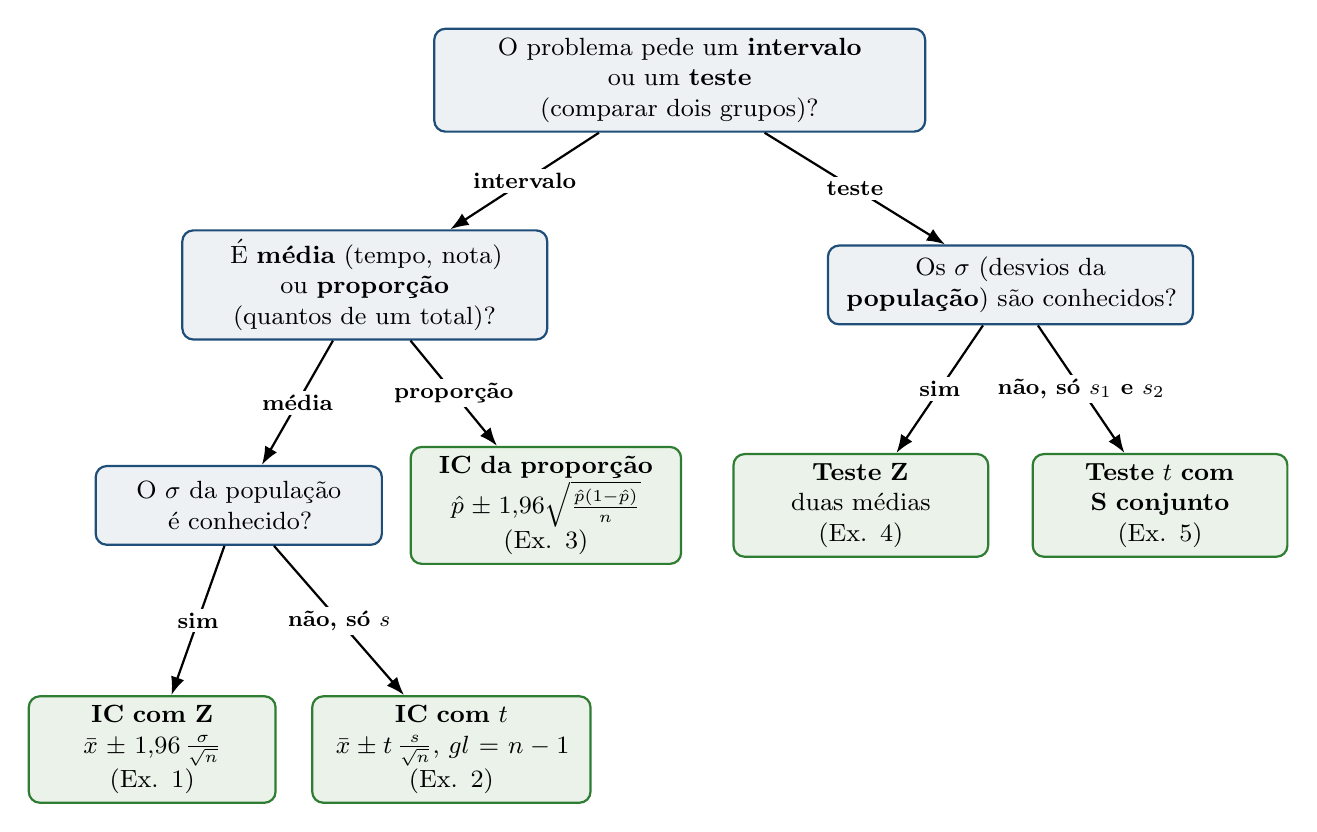
\begin{tikzpicture}[
  perg/.style={draw=azul,thick,fill=azul!8,rounded corners,align=center,minimum height=1cm,font=\small},
  resp/.style={draw=verde,thick,fill=verde!10,rounded corners,align=center,minimum height=1.2cm,font=\small},
  seta/.style={-{Latex},thick},
  lab/.style={font=\footnotesize\bfseries,fill=white,inner sep=1.5pt}]
  \node[perg,text width=6cm] (q1) at (0,0) {O problema pede um \textbf{intervalo}\\ou um \textbf{teste}\\(comparar dois grupos)?};
  \node[perg,text width=4.4cm] (q2) at (-4.0,-2.6) {É \textbf{média} (tempo, nota)\\ou \textbf{proporção}\\(quantos de um total)?};
  \node[perg,text width=4.4cm] (q3) at (4.2,-2.6) {Os $\sigma$ (desvios da\\\textbf{população}) são conhecidos?};
  \node[perg,text width=3.4cm] (q4) at (-5.6,-5.4) {O $\sigma$ da população\\é conhecido?};
  \node[resp,text width=3.2cm] (r3) at (-1.7,-5.4) {\textbf{IC da proporção}\\$\hat p \pm 1,96\sqrt{\frac{\hat p(1-\hat p)}{n}}$\\(Ex. 3)};
  \node[resp,text width=3.0cm] (r4) at (2.3,-5.4) {\textbf{Teste Z}\\duas médias\\(Ex. 4)};
  \node[resp,text width=3.0cm] (r5) at (6.1,-5.4) {\textbf{Teste $t$ com}\\\textbf{S conjunto}\\(Ex. 5)};
  \node[resp,text width=2.9cm] (r1) at (-6.7,-8.5) {\textbf{IC com Z}\\$\bar x \pm 1,96\,\frac{\sigma}{\sqrt n}$\\(Ex. 1)};
  \node[resp,text width=3.3cm] (r2) at (-2.9,-8.5) {\textbf{IC com $t$}\\$\bar x \pm t\,\frac{s}{\sqrt n}$, $gl=n-1$\\(Ex. 2)};
  \draw[seta] (q1) -- node[lab] {intervalo} (q2);
  \draw[seta] (q1) -- node[lab] {teste} (q3);
  \draw[seta] (q2) -- node[lab] {média} (q4);
  \draw[seta] (q2) -- node[lab] {proporção} (r3);
  \draw[seta] (q4) -- node[lab] {sim} (r1);
  \draw[seta] (q4) -- node[lab] {não, só $s$} (r2);
  \draw[seta] (q3) -- node[lab] {sim} (r4);
  \draw[seta] (q3) -- node[lab] {não, só $s_1$ e $s_2$} (r5);
\end{tikzpicture}
\end{center}

\begin{cuidado}
Palavras-chave no enunciado:
\begin{itemize}[leftmargin=*,itemsep=1pt]
  \item ``desvio-padrão \textbf{populacional} conhecido'' ou ``estudos anteriores permitem considerar conhecido'' $\Rightarrow$ use \textbf{Z} (1,96).
  \item ``desvio-padrão \textbf{amostral}'' ou ``populacional \textbf{desconhecido}'' $\Rightarrow$ use \textbf{$t$} de Student.
  \item ``quantos de um total'', ``proporção'', ``percentual'' $\Rightarrow$ \textbf{proporção}.
\end{itemize}
\end{cuidado}

% ================= EXERCÍCIO 1 =================
\newpage
\section*{Exercício 1 -- Intervalo para a média com $\sigma$ conhecido (Z)}
\addcontentsline{toc}{section}{Exercício 1 -- IC para a média com $\sigma$ conhecido}

\begin{enunciado}
Uma equipe de desenvolvimento de software quer estimar o tempo médio necessário para concluir uma tarefa de teste de usabilidade. Em uma amostra aleatória de 64 sessões, o tempo médio foi de 72 minutos. Estudos anteriores permitem considerar conhecido o desvio-padrão populacional de 8 minutos. Construa um intervalo de confiança de 95\% para o tempo médio populacional.
\end{enunciado}

\begin{traducao}
Mediram 64 sessões e a média deu 72 minutos. Queremos uma \textbf{faixa} de valores onde provavelmente está a média \textbf{verdadeira} de todas as sessões.
\end{traducao}

\begin{dados}
\begin{tabular}{ll}
Tamanho da amostra: & $n = 64$ \\
Média da amostra: & $\bar{x} = 72$ minutos \\
Desvio-padrão \textbf{populacional} (conhecido): & $\sigma = 8$ minutos \\
Confiança: & 95\% $\Rightarrow \alpha = 0,05$
\end{tabular}
\end{dados}

\begin{passo}{Passo 2 -- Escolha a distribuição}
O enunciado diz ``desvio-padrão \textbf{populacional} conhecido''. Pelo mapa de decisão: \textbf{Z}.
Para 95\%, o valor crítico é $z = 1,96$.
\[ \text{Fórmula: } \quad IC = \bar{x} \pm 1,96 \times \frac{\sigma}{\sqrt{n}} \]
\end{passo}

\begin{passo}{Passo 3 -- Calcule o erro-padrão}
\[ EP = \frac{\sigma}{\sqrt{n}} = \frac{8}{\sqrt{64}} = \frac{8}{8} = 1,000 \text{ minuto} \]
\end{passo}

\begin{passo}{Passo 4 -- Calcule a margem de erro}
\[ E = 1,96 \times EP = 1,96 \times 1,000 = 1,960 \text{ minuto} \]
\end{passo}

\begin{passo}{Passo 5 -- Calcule os limites}
\[ \text{Limite inferior} = \bar{x} - E = 72 - 1,960 = 70,040 \]
\[ \text{Limite superior} = \bar{x} + E = 72 + 1,960 = 73,960 \]
\end{passo}

\ICline{70,04}{72}{73,96}{1,96}{$\bar x$}

\begin{resultado}
\[ IC_{95\%} = (70,040;\ 73,960) \text{ minutos} \]
\end{resultado}

\begin{interpreta}
Com 95\% de confiança, o tempo médio \textbf{verdadeiro} para concluir a tarefa (considerando todas as sessões, não só as 64) está entre \textbf{70,04 e 73,96 minutos}.
\end{interpreta}

% ================= EXERCÍCIO 2 =================
\newpage
\section*{Exercício 2 -- Intervalo para a média com $s$ ($t$ de Student)}
\addcontentsline{toc}{section}{Exercício 2 -- IC para a média com $t$ de Student}

\begin{enunciado}
Uma equipe de suporte técnico quer estimar o tempo médio de resolução de chamados. Em uma amostra aleatória de 16 chamados, o tempo médio foi de 38,4 minutos e o desvio-padrão amostral foi de 4,8 minutos. O desvio-padrão populacional é desconhecido. Admitindo população aproximadamente normal, construa um intervalo de confiança de 95\% para a média.
\end{enunciado}

\begin{traducao}
É igual ao exercício 1, com uma diferença: agora \textbf{não sabemos} o desvio da população, só o da amostra ($s$). Por isso a régua muda: usamos a tabela $t$, que deixa o intervalo um pouco mais largo (mais ``cauteloso'').
\end{traducao}

\begin{dados}
\begin{tabular}{ll}
Tamanho da amostra: & $n = 16$ \\
Média da amostra: & $\bar{x} = 38,4$ minutos \\
Desvio-padrão \textbf{amostral}: & $s = 4,8$ minutos \\
Graus de liberdade: & $gl = n - 1 = 16 - 1 = 15$
\end{tabular}
\end{dados}

\begin{passo}{Passo 2 -- Escolha a distribuição}
O $\sigma$ é \textbf{desconhecido} $\Rightarrow$ \textbf{$t$ de Student}.
Tabela $t$: linha $gl = 15$, coluna 0,025 $\Rightarrow t = 2,131$.
\[ \text{Fórmula: } \quad IC = \bar{x} \pm t \times \frac{s}{\sqrt{n}} \]
\end{passo}

\begin{passo}{Passo 3 -- Calcule o erro-padrão}
\[ EP = \frac{s}{\sqrt{n}} = \frac{4,8}{\sqrt{16}} = \frac{4,8}{4} = 1,200 \text{ minuto} \]
\end{passo}

\begin{passo}{Passo 4 -- Calcule a margem de erro}
\[ E = t \times EP = 2,131 \times 1,200 = 2,5572 \approx 2,557 \text{ minutos} \]
\end{passo}

\begin{passo}{Passo 5 -- Calcule os limites}
\[ \text{Limite inferior} = 38,4 - 2,557 = 35,843 \]
\[ \text{Limite superior} = 38,4 + 2,557 = 40,957 \]
\end{passo}

\ICline{35,843}{38,4}{40,957}{2,557}{$\bar x$}

\begin{resultado}
\[ IC_{95\%} = (35,843;\ 40,957) \text{ minutos} \]
\end{resultado}

\begin{interpreta}
Com 95\% de confiança, o tempo médio \textbf{verdadeiro} de resolução de chamados está entre \textbf{35,8 e 41,0 minutos} (aproximadamente).
\end{interpreta}

\begin{cuidado}
Não use 1,96 aqui! Só se usa 1,96 quando o $\sigma$ \textbf{da população} é conhecido. E lembre: $gl = n - 1$ (16 chamados dão 15 graus de liberdade, não 16).
\end{cuidado}

% ================= EXERCÍCIO 3 =================
\newpage
\section*{Exercício 3 -- Intervalo para a proporção}
\addcontentsline{toc}{section}{Exercício 3 -- IC para a proporção}

\begin{enunciado}
Uma plataforma de ensino on-line quer estimar a proporção de usuários que concluem o cadastro sem ajuda. Em uma amostra aleatória de 400 usuários, 236 concluíram o cadastro sem assistência. Construa um intervalo de confiança de 95\% para a proporção populacional.
\end{enunciado}

\begin{traducao}
Agora não é tempo nem nota: é ``\textbf{quantos de um total}''. Queremos saber que \textbf{porcentagem} de todos os usuários consegue se cadastrar sozinha.
\end{traducao}

\begin{dados}
\begin{tabular}{ll}
Total da amostra: & $n = 400$ usuários \\
Quantos têm a característica: & $x = 236$ (cadastraram sozinhos) \\
Confiança: & 95\% $\Rightarrow z = 1,96$
\end{tabular}
\end{dados}

\begin{passo}{Passo 2 -- Calcule a proporção da amostra}
\[ \hat{p} = \frac{x}{n} = \frac{236}{400} = 0,590 \quad (= 59\%) \]
O ``resto'' (quem \textbf{não} conseguiu sozinho): $\ 1 - \hat{p} = 1 - 0,590 = 0,410$.
\end{passo}

\begin{passo}{Passo 3 -- Calcule o erro-padrão (devagar, uma conta por vez)}
\[ EP = \sqrt{\frac{\hat{p}\,(1-\hat{p})}{n}} \qquad\text{(a raiz cobre a fração inteira)} \]
\begin{enumerate}[leftmargin=*,itemsep=2pt]
  \item Multiplique: $\ 0,590 \times 0,410 = 0,2419$
  \item Divida por $n$: $\ 0,2419 \div 400 = 0,00060475$
  \item Tire a raiz: $\ \sqrt{0,00060475} = 0,0246 \ (\approx 0,025)$
\end{enumerate}
\end{passo}

\begin{passo}{Passo 4 -- Calcule a margem de erro}
\[ E = 1,96 \times EP = 1,96 \times 0,0246 = 0,0482 \approx 0,048 \]
\small (Use o valor 0,0246, com mais casas. Se usar 0,025 arredondado, dá 0,049 e o resultado fica um pouco diferente do gabarito.)
\end{passo}

\begin{passo}{Passo 5 -- Calcule os limites}
\[ \text{Limite inferior} = 0,590 - 0,048 = 0,542 \quad (54,2\%) \]
\[ \text{Limite superior} = 0,590 + 0,048 = 0,638 \quad (63,8\%) \]
\end{passo}

\ICline{54,2\%}{59\%}{63,8\%}{4,8\%}{$\hat p$}

\begin{resultado}
\[ IC_{95\%} = (0,542;\ 0,638) \quad\text{ou}\quad (54,2\%;\ 63,8\%) \]
\end{resultado}

\begin{interpreta}
Com 95\% de confiança, entre \textbf{54,2\% e 63,8\%} de todos os usuários da plataforma concluem o cadastro sem ajuda.
\end{interpreta}

% ================= TESTES: introdução =================
\newpage
\section*{Antes dos exercícios 4 e 5: o que é um teste de hipóteses?}
\addcontentsline{toc}{section}{Antes dos exercícios 4 e 5: o que é um teste de hipóteses?}

\begin{tcolorbox}[colback=laranja!6,colframe=laranja,title=Analogia do tribunal]
No tribunal, o réu é considerado \textbf{inocente até que se prove o contrário}.
No teste, $H_0$ (``as médias são \textbf{iguais}'') é o ``inocente''. Só ``condenamos'' (rejeitamos $H_0$) se a diferença encontrada for \textbf{grande demais} para ser só acaso.
\end{tcolorbox}

\textbf{Receita do teste (sempre igual):}
\begin{enumerate}[leftmargin=*,itemsep=3pt]
  \item Escreva as hipóteses: $\ H_0: \mu_1 = \mu_2 \ $ (iguais) $\quad$ e $\quad H_1: \mu_1 \neq \mu_2\ $ (diferentes).
  \item Calcule a estatística (Z ou $t$). Ela tem sempre o mesmo formato:
  \[ \text{estatística} = \frac{\text{diferença entre as médias}}{\text{erro-padrão}} \]
  \item Compare com o valor crítico (\textbf{sem olhar o sinal}, ou seja, em módulo $|\ |$):
\end{enumerate}

\begin{center}
\begin{tabular}{ll}
\toprule
Se $|\text{estatística}| > \text{valor crítico}$ & $\Rightarrow$ \textbf{rejeito} $H_0$: as médias \textbf{são diferentes}. \\
Se $|\text{estatística}| \le \text{valor crítico}$ & $\Rightarrow$ \textbf{não rejeito} $H_0$: não há evidência de diferença. \\
\bottomrule
\end{tabular}
\end{center}

O teste é \textbf{bilateral} porque $H_1$ diz só ``diferente'' (pode ser maior ou menor). Então os 5\% ficam divididos: 2,5\% em cada ponta da curva, como no desenho da página 4.

% ================= EXERCÍCIO 4 =================
\newpage
\section*{Exercício 4 -- Teste Z para duas médias ($\sigma$ conhecidos)}
\addcontentsline{toc}{section}{Exercício 4 -- Teste Z para duas médias}

\begin{enunciado}
Uma empresa compara a pontuação média de usabilidade de duas versões independentes de um sistema, em escala de 0 a 100. Na versão A, 50 usuários tiveram média 84; na versão B, 50 usuários independentes tiveram média 79. Considere conhecidos os desvios-padrão populacionais de 10 pontos em cada grupo. Teste, com significância de 5\% e teste bilateral, se as médias populacionais diferem.
\end{enunciado}

\begin{traducao}
A versão A teve nota 84 e a B teve 79. A diferença é 5 pontos. A pergunta é: essa diferença é \textbf{real} ou pode ter sido \textbf{sorte} da amostra?
\end{traducao}

\begin{dados}
\begin{tabular}{lll}
 & \textbf{Versão A (grupo 1)} & \textbf{Versão B (grupo 2)} \\
Tamanho: & $n_1 = 50$ & $n_2 = 50$ \\
Média: & $\bar{x}_1 = 84$ & $\bar{x}_2 = 79$ \\
Desvio \textbf{populacional}: & $\sigma_1 = 10$ & $\sigma_2 = 10$
\end{tabular}
\end{dados}

\begin{passo}{Passo 2 -- Hipóteses e escolha da distribuição}
$H_0: \mu_1 = \mu_2$ (as versões têm a mesma média) $\qquad H_1: \mu_1 \neq \mu_2$ (são diferentes)\\[3pt]
Os $\sigma$ são conhecidos $\Rightarrow$ \textbf{Z}. Valores críticos: $-1,96$ e $+1,96$.
\[ Z = \frac{\bar{x}_1 - \bar{x}_2}{\sqrt{\dfrac{\sigma_1^2}{n_1} + \dfrac{\sigma_2^2}{n_2}}} \]
\end{passo}

\begin{passo}{Passo 3 -- Calcule o erro-padrão (a parte de baixo)}
\begin{enumerate}[leftmargin=*,itemsep=2pt]
  \item Eleve os desvios ao quadrado: $\ \sigma_1^2 = 10^2 = 100 \quad\text{e}\quad \sigma_2^2 = 10^2 = 100$
  \item Divida cada um pelo seu $n$: $\ \dfrac{100}{50} = 2 \quad\text{e}\quad \dfrac{100}{50} = 2$
  \item Some: $\ 2 + 2 = 4$
  \item Tire a raiz: $\ EP = \sqrt{4} = 2,000$
\end{enumerate}
\end{passo}

\begin{passo}{Passo 4 -- Calcule Z (a parte de cima dividida pela de baixo)}
\[ Z = \frac{84 - 79}{2,000} = \frac{5}{2} = 2,500 \]
\end{passo}

\begin{passo}{Passo 5 -- Compare e decida}
$|Z| = 2,500$ \quad é maior que \quad $1,96$ \quad $\Rightarrow$ \quad o Z caiu na \textbf{região vermelha}.
\end{passo}

\RejCurve{1.96}{2.5}{$Z = 2,5$}{1,96}

\begin{resultado}
Como $|Z| = 2,500 > 1,96$, \textbf{rejeita-se $H_0$} ao nível de 5\%.
\end{resultado}

\begin{interpreta}
A diferença de 5 pontos é grande demais para ser só acaso. Há evidência estatística de que as pontuações médias das duas versões \textbf{são diferentes}, e a versão A teve a média maior.
\end{interpreta}

% ================= EXERCÍCIO 5 =================
\newpage
\section*{Exercício 5 -- Teste $t$ com S conjunto ($\sigma$ desconhecidos)}
\addcontentsline{toc}{section}{Exercício 5 -- Teste $t$ com S conjunto}

\begin{enunciado}
Uma equipe compara o tempo médio para completar uma tarefa em duas interfaces independentes. Na interface A, 12 usuários tiveram média de 7,8 minutos e desvio-padrão amostral de 1,2 minuto. Na interface B, 10 usuários tiveram média de 6,5 minutos e desvio-padrão amostral de 1,0 minuto. Considere populações aproximadamente normais, variâncias populacionais desconhecidas e iguais. Usando o desvio-padrão conjunto (S conjunto), teste bilateralmente, com significância de 5\%, se as médias diferem.
\end{enunciado}

\begin{traducao}
Mesma pergunta do exercício 4 (``a diferença é real?''), mas agora só temos os desvios das \textbf{amostras} ($s_1$ e $s_2$). Então: (1) juntamos os dois desvios em um só, o \textbf{S conjunto}, e (2) usamos a tabela \textbf{$t$}.
\end{traducao}

\begin{dados}
\begin{tabular}{lll}
 & \textbf{Interface A (grupo 1)} & \textbf{Interface B (grupo 2)} \\
Tamanho: & $n_1 = 12$ & $n_2 = 10$ \\
Média: & $\bar{x}_1 = 7,8$ & $\bar{x}_2 = 6,5$ \\
Desvio \textbf{amostral}: & $s_1 = 1,2$ & $s_2 = 1,0$ \\
Graus de liberdade: & \multicolumn{2}{l}{$gl = n_1 + n_2 - 2 = 12 + 10 - 2 = 20 \Rightarrow t_{\text{crítico}} = \pm 2,086$}
\end{tabular}
\end{dados}

\begin{passo}{Passo 2 -- Hipóteses e fórmulas}
$H_0: \mu_1 = \mu_2 \qquad H_1: \mu_1 \neq \mu_2$
\[
S_{conj}^2 = \frac{(n_1-1)\,s_1^2 + (n_2-1)\,s_2^2}{n_1+n_2-2}
\qquad\qquad
t = \frac{\bar{x}_1 - \bar{x}_2}{S_{conj}\times\sqrt{\dfrac{1}{n_1}+\dfrac{1}{n_2}}}
\]
\end{passo}

\begin{passo}{Passo 3 -- Calcule o S conjunto (uma conta por vez)}
\begin{enumerate}[leftmargin=*,itemsep=2pt]
  \item Eleve os desvios ao quadrado: $\ s_1^2 = 1,2^2 = 1,44 \quad\text{e}\quad s_2^2 = 1,0^2 = 1,00$
  \item Calcule $n-1$ de cada grupo: $\ 12 - 1 = 11 \quad\text{e}\quad 10 - 1 = 9$
  \item Multiplique: $\ 11 \times 1,44 = 15,84 \quad\text{e}\quad 9 \times 1,00 = 9,00$
  \item Some (parte de cima): $\ 15,84 + 9,00 = 24,84$
  \item Divida pela parte de baixo ($gl = 20$): $\ S_{conj}^2 = 24,84 \div 20 = 1,242$
  \item Tire a raiz: $\ S_{conj} = \sqrt{1,242} = 1,114$
\end{enumerate}
\end{passo}

\begin{passo}{Passo 4 -- Calcule o erro-padrão}
\begin{enumerate}[leftmargin=*,itemsep=2pt]
  \item $\dfrac{1}{12} = 0,0833 \quad\text{e}\quad \dfrac{1}{10} = 0,1000$
  \item Some: $\ 0,0833 + 0,1000 = 0,1833$
  \item Tire a raiz: $\ \sqrt{0,1833} = 0,4282$
  \item Multiplique pelo S conjunto: $\ EP = 1,114 \times 0,4282 = 0,477$
\end{enumerate}
\end{passo}

\begin{passo}{Passo 5 -- Calcule $t$ e decida}
\[ t = \frac{7,8 - 6,5}{0,477} = \frac{1,3}{0,477} \approx 2,724 \]
$|t| = 2,724$ \quad é maior que \quad $2,086$ \quad $\Rightarrow$ \quad caiu na \textbf{região vermelha}.\\
{\small (Se aparecer 2,725 na sua calculadora, é só arredondamento: a conclusão é a mesma.)}
\end{passo}

\RejCurve{2.086}{2.724}{$t = 2,724$}{2,086}

\begin{resultado}
Como $|t| = 2,724 > 2,086$, \textbf{rejeita-se $H_0$} ao nível de 5\%.
\end{resultado}

\begin{interpreta}
A diferença de 1,3 minuto entre as interfaces não parece ser acaso. Há evidência de que os tempos médios \textbf{são diferentes}: a interface A leva mais tempo (7,8 min contra 6,5 min).
\end{interpreta}

\begin{cuidado}
\begin{itemize}[leftmargin=*,itemsep=1pt]
  \item Na fórmula do S conjunto, multiplique pelo \textbf{desvio ao quadrado} ($s^2$), não pelo desvio.
  \item Depois de dividir por 20, \textbf{não esqueça a raiz}: $S_{conj} = 1,114$, não 1,242.
  \item Aqui $gl = n_1 + n_2 - 2 = 20$ (e não $n - 1$).
\end{itemize}
\end{cuidado}

% ================= RESUMO =================
\newpage
\section*{Folha-resumo para levar na cabeça}
\addcontentsline{toc}{section}{Folha-resumo}

\renewcommand{\arraystretch}{1.6}
\begin{center}
\begin{tabular}{>{\raggedright\arraybackslash}m{3.6cm} >{\centering\arraybackslash}m{6.2cm} >{\raggedright\arraybackslash}m{5.2cm}}
\toprule
\textbf{Situação} & \textbf{Fórmula} & \textbf{Valor crítico (95\%)} \\
\midrule
IC média, $\sigma$ conhecido & $\bar x \pm z\,\dfrac{\sigma}{\sqrt n}$ & $z = 1,96$ \\
IC média, só $s$ & $\bar x \pm t\,\dfrac{s}{\sqrt n}$ & tabela $t$, $gl = n-1$ \\
IC proporção & $\hat p \pm z\sqrt{\dfrac{\hat p(1-\hat p)}{n}}$ & $z = 1,96$ \\
Teste Z, 2 médias & $Z=\dfrac{\bar x_1-\bar x_2}{\sqrt{\frac{\sigma_1^2}{n_1}+\frac{\sigma_2^2}{n_2}}}$ & $\pm 1,96$ \\
Teste $t$, S conjunto & $t=\dfrac{\bar x_1-\bar x_2}{S_{conj}\sqrt{\frac1{n_1}+\frac1{n_2}}}$ & tabela $t$, $gl=n_1+n_2-2$ \\
\bottomrule
\end{tabular}
\end{center}

\begin{tcolorbox}[colback=verde!8,colframe=verde,title=Resultados da lista (confira os seus)]
\begin{tabular}{ll}
Ex. 1: & $EP = 1$; $\ E = 1,96$; $\ IC = (70,040;\ 73,960)$ minutos \\
Ex. 2: & $EP = 1,2$; $\ E = 2,557$; $\ IC = (35,843;\ 40,957)$ minutos \\
Ex. 3: & $\hat p = 0,59$; $\ EP \approx 0,025$; $\ E = 0,048$; $\ IC = (54,2\%;\ 63,8\%)$ \\
Ex. 4: & $EP = 2$; $\ Z = 2,500 > 1,96$ $\Rightarrow$ rejeita $H_0$ \\
Ex. 5: & $S_{conj} = 1,114$; $\ EP = 0,477$; $\ t = 2,724 > 2,086$ $\Rightarrow$ rejeita $H_0$
\end{tabular}
\end{tcolorbox}

\begin{tcolorbox}[colback=azul!5,colframe=azul,title=Checklist na hora da prova]
\begin{enumerate}[leftmargin=*,itemsep=1pt]
  \item Sublinhei no enunciado: $n$, média, desvio e se o desvio é \textbf{populacional} ou \textbf{amostral}?
  \item Escolhi Z ou $t$ pelo mapa de decisão?
  \item Se for $t$: calculei os $gl$ certos?
  \item Fiz uma conta por vez, com 4 casas, e só arredondei no fim?
  \item Escrevi a \textbf{interpretação em palavras}, com a unidade (minutos, \%, pontos)?
\end{enumerate}
\end{tcolorbox}

\end{document}
